
\index{Godde, Ben}

\paragraph{Research Team}
Ben Godde (Professor), Claudia Voelcker-Rehage (Postdoctoral Fellow), Mikhail Babanin (Doctoral Fellow), Alexander Knop (Diploma Student, University of Bremen).

First, within the sensory domain we are interested in the plastic-adaptive competencies related to tactile processing of younger and older adults. Using functional MRI and psychophysics we investigate the cortical topography of tactile perception and the cortical mechanisms of perceptual learning.
	
	Second, within the motor domain, we are mainly interested in upper extremity force control. Control of the fine finger forces is an elementary component of movement production of many daily activities (e.g. dressing, eating, opening containers) and its assessment provides insight into movement control and coordination. A decline in force control is common in older adults. We examine age-related differences in force control, practice effect on force modulation, and age-related differences in dual-task performance. Besides force control we are interested in the intermanual transfer of learned motor programs.
	
	In a third line of research we are going to focus on the interaction between motor and sensory performance. Particularly, we are interested in the following questions: (1) Does high frequency tactile stimulation help to diminish age-related performance decrements in force control? 
	
\newpage
(2) Does high frequency tactile stimulation facilitate sensory and/or motor learning? These questions are the first steps in developing appropriate interventions to improve manual dexterity in older adults.

\null
\textbf{Research Highlights 2006}


\textit{Effects of high frequency tactile stimulation on sensory and motor performance in younger and older adults}

	It is assumed that an important mechanism responsible for precise force control is tactile sensitivity. However, also contradictory results exist and the neural control mechanisms responsible for precise manipulation of grasping forces are largely unknown. We examined the link between motor and tactile domains by applying an intervention paradigm of high frequency ($\sim$20Hz) tactile stimulation (tHFS). This protocol is assumed to induce long-term potentiation (LTP) like effects in the neocortex and has recently been shown to profoundly improve tactile acuity. 

	Younger (18-28 years of age) and older (65-75 years of age) right handed participants were randomly assigned to an experimental and a control group. Before and after 30 minutes of tHFS on the index finger and thumb of the left hand, participants performed different tactile (spatial and temporal discrimination) and motor tasks (unimanual isometric precision grip task using a Mini Model force transducer and Purdue Pegboard test) with their stimulated fingers.
	
	Results indicated that tHFS significantly improved tactile frequency discrimination of the left index finger, whereas motor performance as assessed with the pegboard task was impaired (see Figure \ref{fig:profBenGodde}). These effects were found for both age groups with similar effect sizes even though absolute levels of performance in all tasks were lower for older as compared to younger adults. For the precision grip task younger subjects of both the experimental and control group similarly improved from the pre to the post test. Contrary, only older subjects which received the tHFS intervention could profit from the test repetition whereas the performance of the older control group remained stable. 
	
	Our results suggest that reorganization of the somatosensory cortex presumably induced by the applied protocol of passive tactile stimulation not only promotes sensory performance but also significantly affects fine motor control of the respective fingers. Moreover, our study reveals the remaining plastic capacity of the older brain (Voelcker-Rehage, Knop, Babanin \& Godde, 2006). 

%\begin{figure}[ht]
%  \begin{center}
%    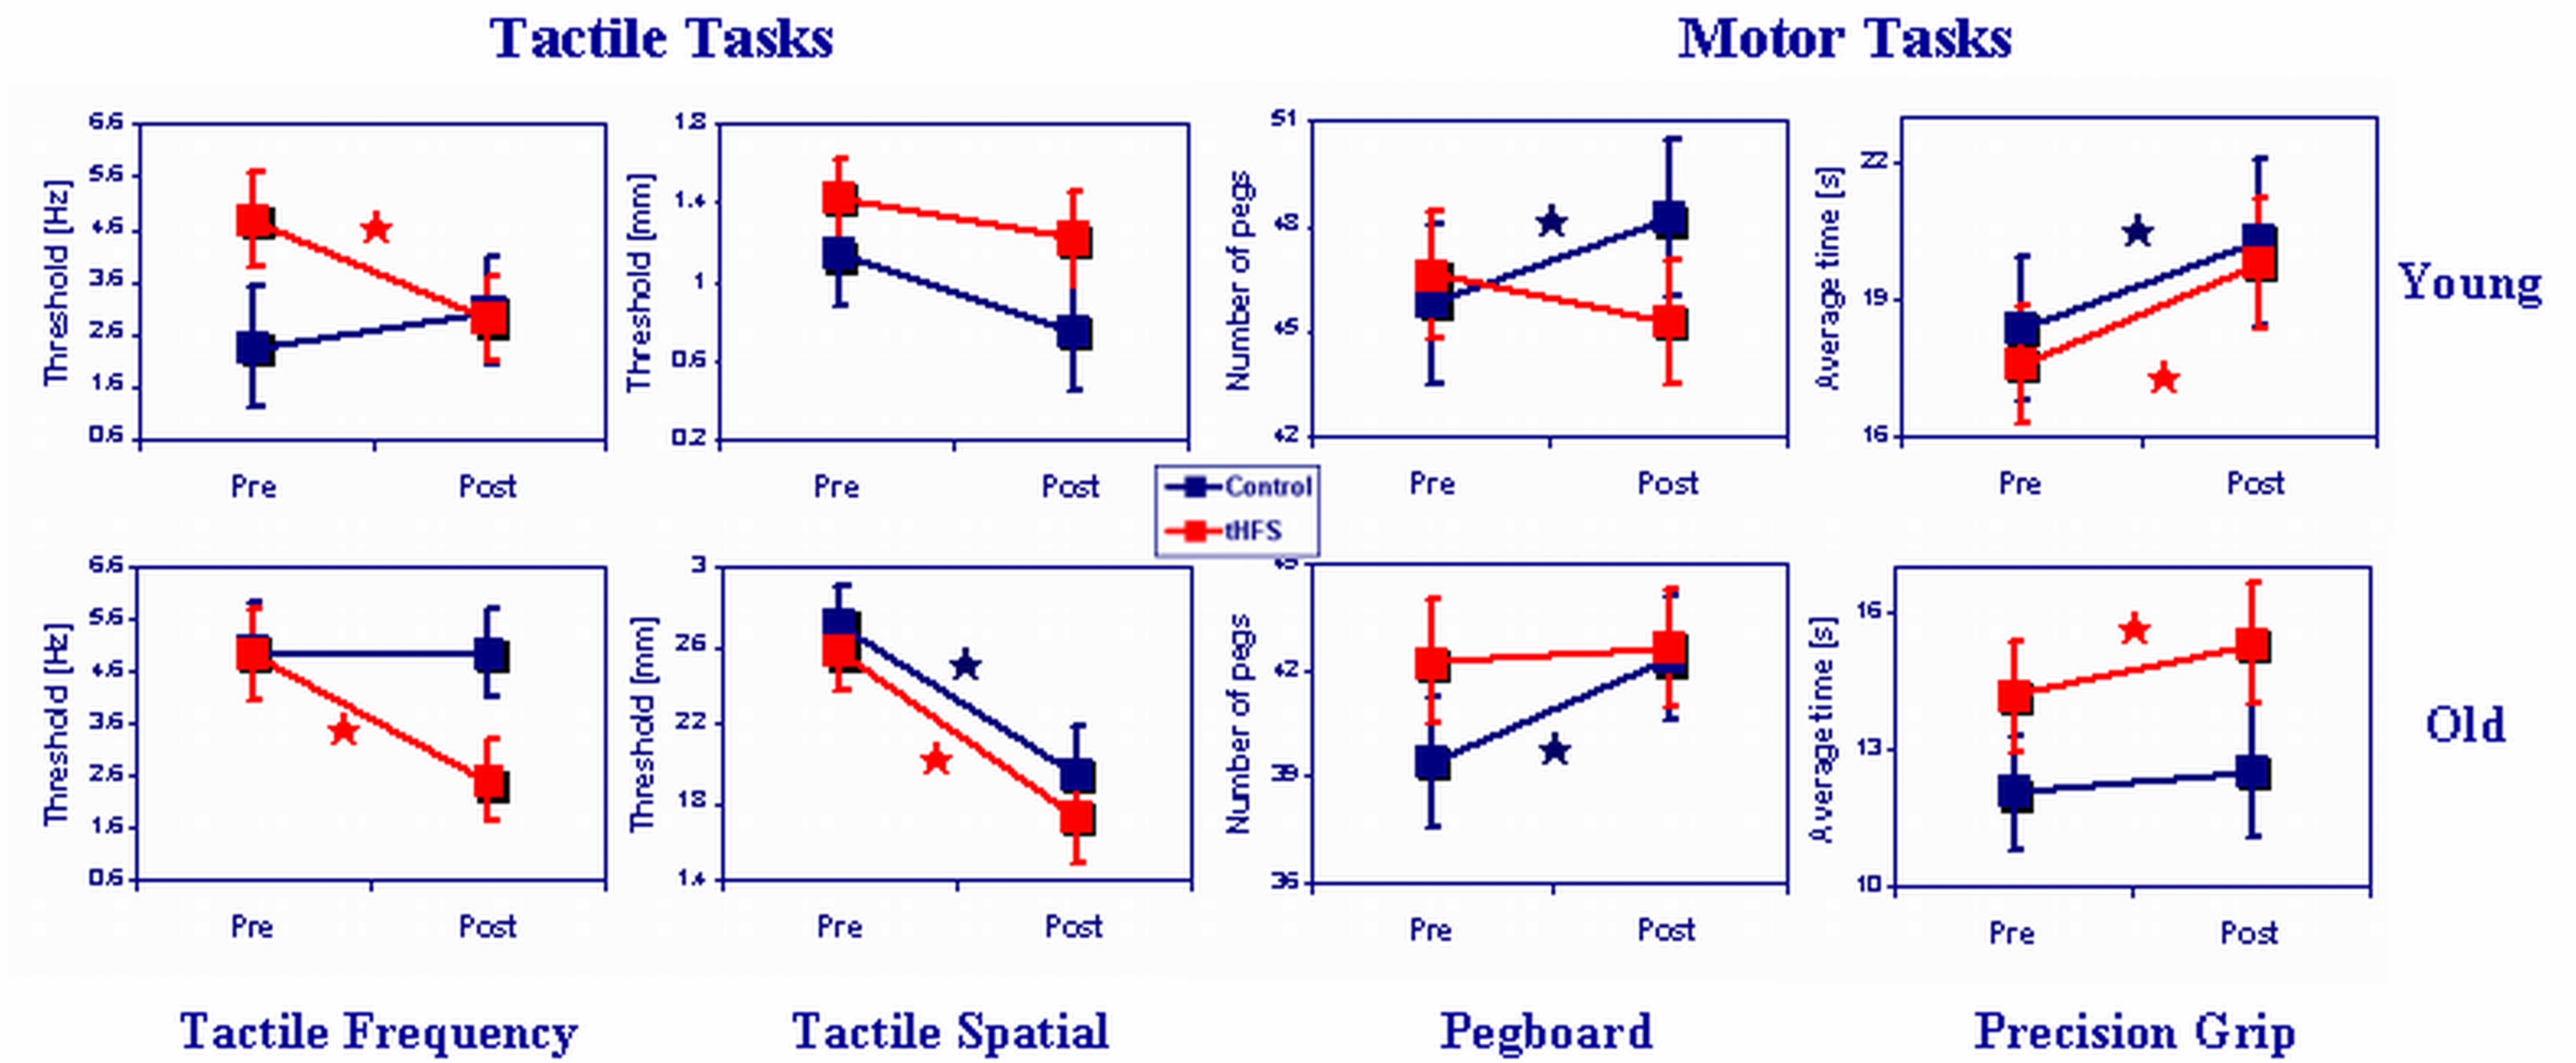
\includegraphics[width=7.5cm]{profBenGodde-fig1.jpg}
%    \caption{Differential effects of tHFS on tactile (left 2 columns) and motor (right 2 columns) performance in young %(top) and old (bottom) subjects. Experimental group shown in red, control group in blue.}\label{fig:profBenGodde}
%   \end{center}
%\end{figure}

\begin{figure}[htb]
  \begin{center}
    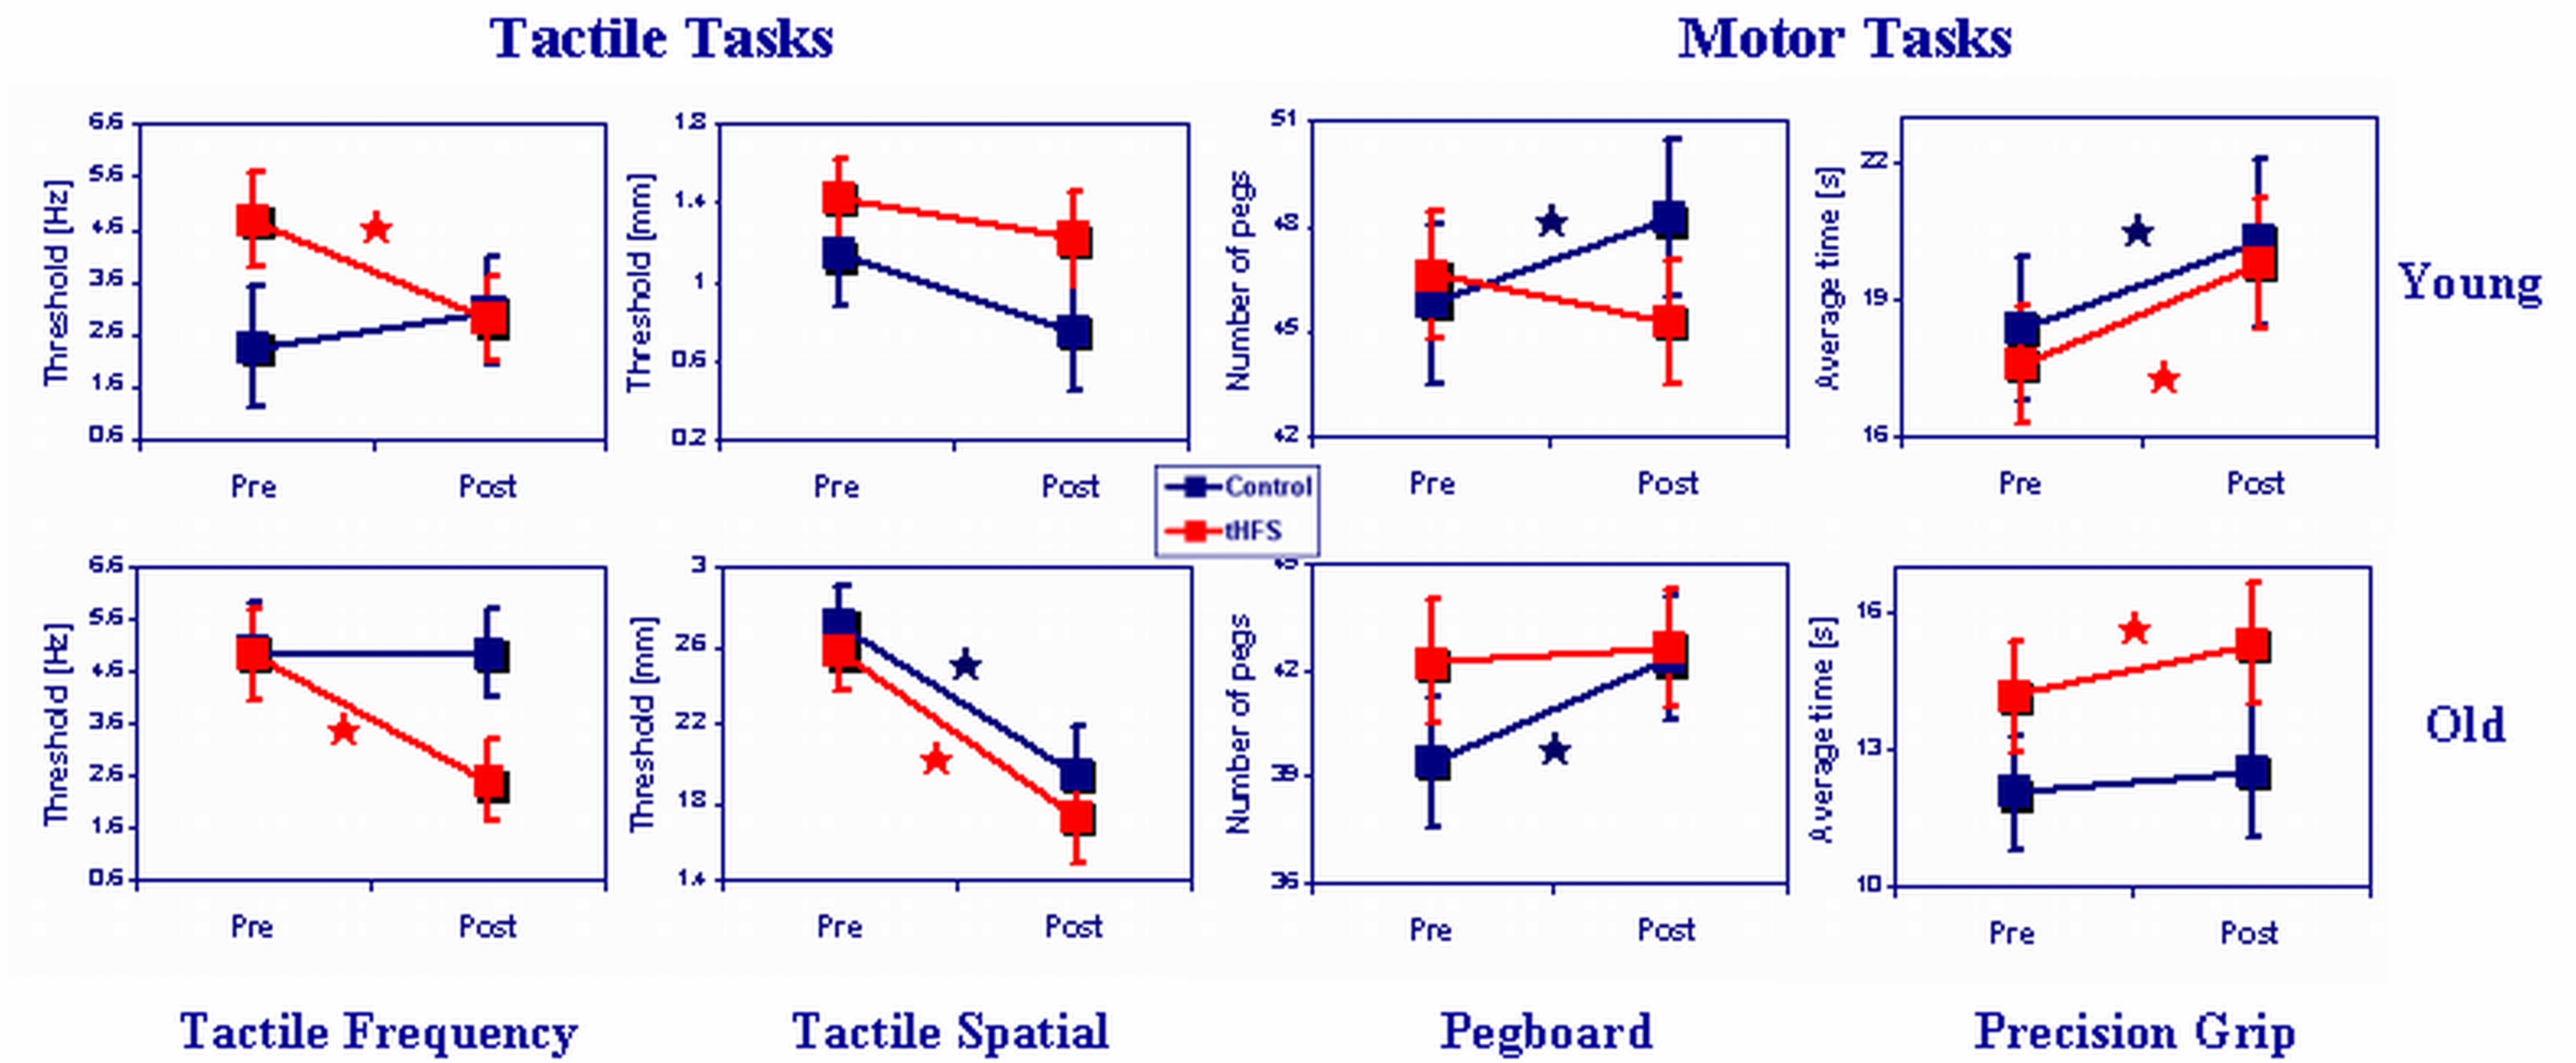
\includegraphics[width=0.5\textwidth]{profBenGodde-fig1}
    \caption{Differential effects of tHFS on tactile (left 2 columns) and motor (right 2 columns) performance in young (top) and old (bottom) subjects. Experimental group shown in red, control group in blue.}
    \label{fig:profBenGodde}
  \end{center}
\end{figure}




\enlargethispage*{0.2cm}
\paragraph{Collaborations}
\begin{itemize}
\item University Hospital T\"{u}bingen \\ MEG-Center \\ PD Dr. Christoph Braun 
\item University of T\"{u}bingen \\ Medical Psychology and Behavioral Neurobiology \\ Dipl-Psych. Ahmed A. Karim
\item International School for Advanced Studies \\ Trieste, Italy \\ Cognitive Neuroscience Sector \\ Prof. Mathew E. Diamond, PhD
\item Lerner Research Institute, USA \\ Department of Biomedical Engineering \\ Cleveland Clinic Foundation \\ Jay L. Alberts, PhD
\item IUB, SES \\ Prof. Dr. Claus Hilgetag
\item University of Bremen \\ Interdisciplinary Center for Cognitive Sciences \\ Prof. Dr. Manfred Herrmann; Prof. Dr. Manfred Fahle
\end{itemize}

\begin{bibunit}[apalike]
\nocite{*}
\putbib[profBenGodde1]
\end{bibunit}

\paragraph{Grants}
\begin{itemize}
\item DFG (submitted; PI: C. Voelcker-Rehage in cooperation with Jay L. Alberts, PhD, Cleveland Clinic Foundation, USA): Age-related changes in functional uni- and bimanual dexterity; grasping force modulation in older adults.

\item BMBF (PI: JCLL). B. Godde, C. Voelcker-Rehage: subproject ``Adaptive Competence'' within the joint research project ``Effects of Matches/Mismatches between Aspects of Human and Social Capital, Corporate Strategy and Work Organization on the Physical and Mental Well-Being of Employees''. 
 
\end{itemize}